testfile{pgfplotstest.ternary.tex}
\testsection{Ternary axes}

\testsubsection{About the structure; first steps}
\begin{tikzpicture}
%\tracingmacros=2 \tracingcommands=2
	\begin{ternaryaxis}[
		extra description/.add code={}{%
			\pgfpathcircle
				{\pgfplotsqpointoutsideofaxis{v00}{1}{15pt}}%
				{5pt}%
			\pgfusepath{fill}%
			\pgfpathcircle
				{\pgfplotsqpointoutsideofaxis{0v0}{0.5}{15pt}}%
				{5pt}%
			\pgfusepath{fill}%
			\pgfpathcircle
				{\pgfplotsqpointoutsideofaxis{00v}{0.5}{15pt}}%
				{5pt}%
			\pgfusepath{fill}%
		},
	]

\def\markpoint(#1);{%
	\node[anchor=base,draw=black,font=\tiny] at (axis cs:#1) {(#1)};
	\filldraw (axis cs:#1) circle(0.5pt);
}

	\addplot3[only marks,scatter,point meta=\coordindex] coordinates {
		(1,0,0)
	%	(0,1,0)
		(0,0,1)
		(1,0,1)
	%	(0,0.5,0.5)
	%	(0.5,0.5,0)
	%	(0.5,0,0.5)
	%	(0.33333,0.33333,0.33333)
	};
	%--------------------------------------------------
	% \draw[red] 
	% 	(axis cs:1,0,0) -- 
	% 	(axis cs:0,1,0) --
	% 	(axis cs:0,0,1) -- cycle;
	%-------------------------------------------------- 

		\markpoint(0.8,0,0.2);
		\markpoint(0.8,0.2,0);
		\markpoint(0,0.8,0.2);

		\markpoint(0.2,0,0.8);
		\markpoint(0.2,0.8,0);
		\markpoint(0,0.2,0.8);
	\end{ternaryaxis}
\end{tikzpicture}

\testsubsection{Only the axis, default params}
\begin{tikzpicture}
%\tracingmacros=2 \tracingcommands=2
	\begin{ternaryaxis}[
	]

	\addplot3[only marks,scatter,point meta=\coordindex] coordinates {
		(1,0,0)
		(0,1,0)
		(0,0,1)
		(1,0,1)
		(0,0.5,0.5)
		(0.5,0.5,0)
		(0.5,0,0.5)
		(0.33333,0.33333,0.33333)
	};
	\end{ternaryaxis}
\end{tikzpicture}

\testsubsection{Labels + 2 minor grid lines}
\begin{tikzpicture}
%\tracingmacros=2 \tracingcommands=2
	\begin{ternaryaxis}[
		title=A Title,
		xlabel=xlabel,
		ylabel=ylabel,
		zlabel=zlabel,
		minor tick num=2,
		grid=both,
	]

	\addplot3[only marks,scatter,point meta=\coordindex] coordinates {
		(1,0,0)
		(0,1,0)
		(0,0,1)
		(1,0,1)
		(0,0.5,0.5)
		(0.5,0.5,0)
		(0.5,0,0.5)
		(0.33333,0.33333,0.33333)
	};
	\end{ternaryaxis}
\end{tikzpicture}

\testsubsection{Sloped labels}
\begin{tikzpicture}
%\tracingmacros=2 \tracingcommands=2
	\begin{ternaryaxis}[
		title=A Title,
		xlabel=xlabel,
		ylabel=ylabel,
		zlabel=zlabel,
		label style={sloped},
	]

	\addplot3[only marks,scatter,point meta=\coordindex] coordinates {
		(1,0,0)
		(0,1,0)
		(0,0,1)
		(1,0,1)
		(0,0.5,0.5)
		(0.5,0.5,0)
		(0.5,0,0.5)
		(0.33333,0.33333,0.33333)
	};
	\end{ternaryaxis}
\end{tikzpicture}

\testsubsection{Scaling with footnotesize; extra y ticks}
\begin{tikzpicture}
%\tracingmacros=2 \tracingcommands=2
	\begin{ternaryaxis}[
		footnotesize,
		extra y ticks=0.44,
	]

	\addplot3+[scatter] coordinates {
		(1,0,0)
		(0,1,0)
		(0,0,1)
		(1,0,1)
		(0,0.5,0.5)
		(0.5,0.5,0)
		(0.5,0,0.5)
		(0.33333,0.33333,0.33333)
	};
	\end{ternaryaxis}
\end{tikzpicture}

\testsubsection{Legends}
\begin{tikzpicture}
%\tracingmacros=2 \tracingcommands=2
	\begin{ternaryaxis}[
		legend entries={First,Second},
	]

	\addplot3+[scatter] coordinates {
		(1,0,0)
		(0,1,0)
		(0,0,1)
		(1,0,1)
		(0,0.5,0.5)
		(0.5,0.5,0)
		(0.5,0,0.5)
		(0.33333,0.33333,0.33333)
	};

	\addplot3 coordinates {
		(0.1,0.5,0.4)
		(0.2,0.5,0.3)
		(0.3,0.6,0.1)
	};
	\end{ternaryaxis}
\end{tikzpicture}


\testsubsection{ternary limits relative=false}
\begin{tikzpicture}
%\tracingmacros=2 \tracingcommands=2
	\begin{ternaryaxis}[
		xmin=0,xmax=50,
		ymin=0,ymax=200,
		zmin=0,zmax=300,
		ternary limits relative=false,
	]

	\addplot3 coordinates {
		(40,80,100)
		(30,50,110)
		(20,50,120)
	};
	\end{ternaryaxis}
\end{tikzpicture}

\testsubsection{Special annotations in cartesian coords}
\begin{tikzpicture}
%\tracingmacros=2 \tracingcommands=2
	\begin{ternaryaxis}[
		clip=false,
	]

	\addplot3 coordinates {
		(0.1,0.5,0.4)
		(0.2,0.5,0.3)
		(0.3,0.6,0.1)
	};

	\node[fill=white,draw] at (0,0) {$y (0,0)$};
	\node[fill=white,draw] at (1,0) {$z (1,0)$};
	\node[fill=white,draw] at (0.5,{sqrt(3)/2}) {$x (\frac12,\frac{\sqrt3}{2})$};
	\end{ternaryaxis}
\end{tikzpicture}

\testsubsection{Special annotations in description cs}
\begin{tikzpicture}
%\tracingmacros=2 \tracingcommands=2
	\begin{ternaryaxis}[
		extra description/.append code={
			\node[fill=white,draw] at (0,0) {$y (0,0)$};
			\node[fill=white,draw] at (1,0) {$z (1,0)$};
			\node[fill=white,draw] at (0.5,1) {$x (0.5,1)$};
		},
	]

	\addplot3 coordinates {
		(0.1,0.5,0.4)
		(0.2,0.5,0.3)
		(0.3,0.6,0.1)
	};

	\end{ternaryaxis}
\end{tikzpicture}

\testsubsection{Only part of axis FIXME}
Needs more logic in pgfplots, I fear

\begin{tikzpicture}
\begin{ternaryaxis}[
	xmax=100,ymax=100,zmax=100,
	ternary limits relative=false,
	%ternary start x=0.5,
	xlabel=Water,
	ylabel=D--Threonine,
	zlabel=L--Threonine,
	label style={sloped}
]
	\addplot3 coordinates {
		(82,	18,	0)
		(75,	17,	8)
		(77,	12,	11)
		(75,	8,	17)
		(81,	0,	19)
	};
	\addplot3 coordinates {
		(75,	25,	0)
		(69,	25,	6)
		(64,	24,	12)
		(65.5,	23,	11.5)
		(67,	17,	16)
		(66,	12,	22)
		(64,	11,	25)
		(69,	5,	26)
		(76,	1,	23)
	};
	\legend{$10$, $20$}
\end{ternaryaxis}
\end{tikzpicture}

\testsubsection{Scaling with yscale=2 FIXME}
\begin{tikzpicture}
%\tracingmacros=2 \tracingcommands=2
	\begin{ternaryaxis}[
		legend entries={First,Second},
		yscale=2,
	]

	\addplot3+[scatter] coordinates {
		(1,0,0)
		(0,1,0)
		(0,0,1)
		(1,0,1)
		(0,0.5,0.5)
		(0.5,0.5,0)
		(0.5,0,0.5)
		(0.33333,0.33333,0.33333)
	};

	\addplot3 coordinates {
		(0.1,0.5,0.4)
		(0.2,0.5,0.3)
		(0.3,0.6,0.1)
	};
	\end{ternaryaxis}
\end{tikzpicture}


\testsubsection{reversed axes}
\begin{tikzpicture}
%\tracingmacros=2 \tracingcommands=2
	\begin{ternaryaxis}[
		title=Normal Direction,
		axis line style={-stealth},
		separate axis lines,
		xlabel=xlabel,
		ylabel=ylabel,
		zlabel=zlabel,
	]

	\addplot3 coordinates {
		(0.1,0.5,0.4)
		(0.2,0.5,0.3)
		(0.3,0.6,0.1)
	};

	\end{ternaryaxis}
\end{tikzpicture}

\begin{tikzpicture}
%\tracingmacros=2 \tracingcommands=2
	\begin{ternaryaxis}[
		title=Reversed,
		x dir=reverse,
		y dir=reverse,
		z dir=reverse,
		axis line style={-stealth},
		separate axis lines,
		xlabel=xlabel,
		ylabel=ylabel,
		zlabel=zlabel,
	]

	\addplot3 coordinates {
		(0.1,0.5,0.4)
		(0.2,0.5,0.3)
		(0.3,0.6,0.1)
	};

	\end{ternaryaxis}
\end{tikzpicture}


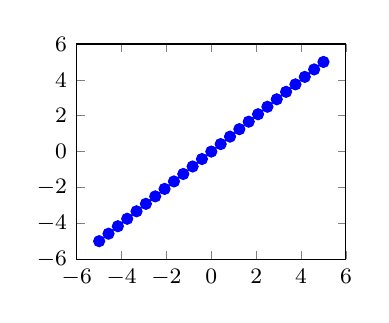
\begin{tikzpicture}
	\begin{axis}[footnotesize]
		\addplot {x};
	\end{axis}
\end{tikzpicture}
